%ffalse
\let\negmedspace\undefined
\let\negthickspace\undefined
\documentclass[journal,12pt,onecolumn]{IEEEtran}
\usepackage{cite}
\usepackage{amsmath,amssymb,amsfonts,amsthm}
\usepackage{algorithmic}
\usepackage{graphicx}
\usepackage{textcomp}
\usepackage{xcolor}
\usepackage{txfonts}
\usepackage{listings}
\usepackage{enumitem}
\usepackage{mathtools}
\usepackage{gensymb}
\usepackage{comment}
\usepackage[breaklinks=true]{hyperref}
\usepackage{tkz-euclide} 
\usepackage{listings}
\usepackage{gvv}                                        
%\def\inputGnumericTable{}                                 
\usepackage[latin1]{inputenc}                                
\usepackage{color}                                            
\usepackage{array}                                            
\usepackage{longtable}                                       
\usepackage{calc}                                             
\usepackage{multirow}                                         
\usepackage{hhline}                                           
\usepackage{ifthen}                                           
\usepackage{lscape}
\usepackage{tabularx}
\usepackage{array}
\usepackage{float}


\newtheorem{theorem}{Theorem}[section]
\newtheorem{problem}{Problem}
\newtheorem{proposition}{Proposition}[section]
\newtheorem{lemma}{Lemma}[section]
\newtheorem{corollary}[theorem]{Corollary}
\newtheorem{example}{Example}[section]
\newtheorem{definition}[problem]{Definition}
\newcommand{\BEQA}{\begin{eqnarray}}	
\newcommand{\EEQA}{\end{eqnarray}}
\newcommand{\define}{\stackrel{\triangle}{=}}
\theoremstyle{remark}
\newtheorem{rem}{Remark}

% Marks the beginning of the document
\begin{document}
\bibliographystyle{IEEEtran}
\vspace{3cm}

\title{18/A/E/36-49}
\author{AI24BTECH11011 - HIMANI GOURISHETTY}
\maketitle
\bigskip

\renewcommand{\thefigure}{\theenumi}
\renewcommand{\thetable}{\theenumi}

\begin{enumerate}
\item Let $C_1$ and $C_2$ be the graphs of the functions $y=x^2$ and $y=2x$, $0\le x\le1$ respectively. Let $C_3$ be graph of a function  y=$f\brak{x}$, $0\le x \le 1$, $f\brak{0}$=0. For a point $\vec{P}$ on $C_1$, let the lines through $\vec{P}$, parallel to the axes, meet $C_2$and $C_3$ at $\vec{Q}$ and $\vec{R}$ respectively(see figure). If for every position of $\vec{P}$ (on $C_1$), the areas of the shaded regions $OPQ$ and $ORP$ are equal, determine the function of $f\brak{x}$.
\hfill{(1998-8 Marks)}
\begin{figure}[h!]
\centering
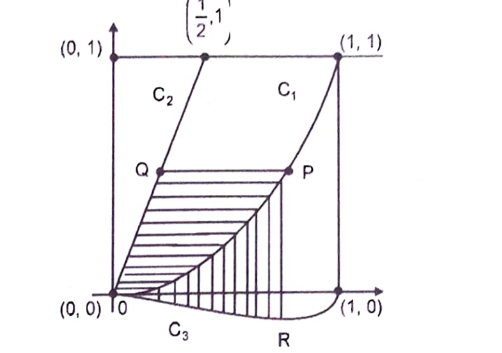
\includegraphics[width=0.7\linewidth]{figs/fig1.png}
\label{fig:11011}
\end{figure}
\item Integrate $\int_{0}^{\pi}\frac{e^{\cos{x}}}{e^{\cos{x}}+e^{-\cos{x}}}dx$
 \hfill{(1999-2 Marks)}\\	      			
\item Let $f\brak{x}$ be a continuos function given by 
	\begin{align}
	f\brak{x} &=
	\begin{cases}
	2x, \abs{x}\le1\\
	x^2+ax+b, \abs{x}>1
	\end{cases}
	\end{align}
\item Find the area of the region in the third quadrant bounded by the curves $x=-2y^2$ and $y=f\brak{x}$ lying on the left of the line $8x+1=0$. 						
\hfill{(1999-10marks)}\\
\item For $x > 0 $, $let $f\brak{x}$=\int_{e}^{x}\frac{\ln{t}}{1+t}dx$.Find the function $f\brak{x} + f\brak{\frac{1}{x}}$
 and show that $f\brak{e}+f\brak{\frac{1}{e}}=
\frac{1}{2}$. Here, $\ln{t}$=$\log{t}$.
\hfill{(2000-5Marks)}
\item Let $b\neq0$ and for $j=0, 1, 2, \dots{...}, n$, $S_j$ be the area of the region bounded by the y-axis and the curve $xe^{ay}$ = sin by $\frac{jr}{b} \le y \le \frac{(j+1)\pi}{b}$. Show that  $S_0,S_1,S_2,......,S_n$ are in geometric progression. Also, find their sum for $a=-1$ and $b= \pi$. \\.
\hfill{(2001-5Marks)}
\item Find the area of the region bounded by the curves $y=x^2$, $y=\abs{2-x}$ and $y=2$, which lies to the right of the line $x=1$\\. 
\hfill{(2002-5 Marks)}
\item If f is an even function then prove that 	$\int_{0}^{\frac{\pi}{2}}f(\cos{2x})\cos{x}dx$ =$\sqrt{2}\int_{0}^{\frac{\pi}{4}}f\brak{\sin{2x}}\cos{x}dx$\\.
\hfill{(2003-2Marks)}
\item If $y(x)=\int_{\frac{\pi^2}{16}}^{x^2}\frac{\cos{x}\cos{\sqrt{\theta}}}{1+\sin^2{\sqrt{\theta}}}dx$, then find $\frac{dy}{dx}$ at $x=\pi$\\.
\hfill{(2004-2Marks)}
\item  Find the value of $\int_{\frac{-\pi}{3}}^{\frac{\pi}{3}}\frac{\pi+4x^3}{2-\cos{(\abs{x}+\frac{\pi}{3})}}dx$\\.
\hfill{(2004-4Marks)}
\item Evaluate $\int_{0}^{\pi}e^{\cos{x}}\brak{(2\sin{(\frac{1}{2}\cos{x}})+3\cos{(\frac{1}{2}\cos{x})})\sin{x}}dx$\\.
\hfill{(2005-2Marks)}
\item Find the area bounded by the curves \\  
$x^2=y,x^2=-y$ and $y^2=4x-3$
\hfill{(2005-4Marks)}
\item  $f\brak{x}$ is a differentiable function and $g\brak{x}$ is  double differentiable function such that $f\brak{x}\le1$ and $f^{\prime}\brak{x}=g\brak{x}$. if $f^2\brak{0}+g^2\brak{0}=9$. Prove that there exist some $c\in(-3,3)$ such that $g\brak{c}.g^{\prime}\brak{c}<0$.\\.
\hfill{(2005-6Marks)}
\item 
  \[
\myvec{ 4a^2 & 4a & 1\\4b^2 & 4b & 1\\4c^2 & 4c & 1}
\myvec{f\brak{-1}\\f\brak{1}\\f\brak{2}} =
\myvec{3a^2+3a\\3b^2+3b\\3c^2+3c}
\]
$f\brak{x}$ is a quadratic function and its maximum value occurs at a point $\vec{V}$. $\vec{A}$ is a point of intersection of y=$f\brak{x}$ with x axis and point $\vec{B}$ is such that chord $AB$ subtends a right angle at $\vec{V}$. Find the area enclosed by $f\brak{x}$ and chord $AB$. 
\hfill{(2005-6Marks)}
\item The value of $5050 \frac{\int_{0}^{1}(1-x^50)^100}{\int{0}^{1} {(1-x^50)^101}}dx$
\hfill{(2006-6M)}


\end{enumerate}


\end{document}
